% arara: xelatex: {synctex: true}
% arara: indent: {overwrite: yes}
\documentclass[]{IMTexam}

\usepackage{IMTtikz}

\givecredits
\author{Isabella B.}
\USPN{11810773}
\date{}
\lecture{Física I} % disciplina
\lcode{4302111}
\hwtype{Resolução} % o que é
\examname{Lista 2} % prova

\begin{document}

\maketitle

\begin{questions}

	\question
	Uma lâmpada pende sobre o centro de uma mesa redonda de raio $ r $. A que altura da mesa deve estar a lâmpada para que a iluminação de um objeto que se encontra à beira da mesa seja a melhor possível? A iluminação é diretamente proporcional ao cosseno do ângulo de incidência da luz (que se propaga em linha reta) e inversamente proporcional ao quadrado da distância da fonte (lâmpada).

	\begin{solution}

		\begin{multi}
			Pelo enunciado, sabemos que a intensidade de iluminação $ I\propto \dfrac{\cos\theta}{\ell^{2}} $. Sendo $ \theta $ o ângulo de incidência, $ \cos\theta=\dfrac{h}{\ell} $ e $ \ell=(r^{2}+h^{2})^{1/2} $. Para encontrar o valor ótimo que a questão pede devemos: \begin{enumerate}
				\item colocar $ I $ em função de alguma das variáveis do problema ($ h $ é uma boa candidata, pois é exatamente o que queremos), e;
				\item derivar e igualar a zero, para encontrar o valor ótimo.
				\item[(extra)] caso haja mais de uma resposta para o item 2, devemos derivar $ I $ novamente para encontrar qual dos dois valores se encaixa nas especificações do problema (melhor iluminação $ \implies I$ máximo, logo $ I^{\prime\prime}(h_{\text{máx}})<0 $).
			\end{enumerate}

			\nextcol

			\centering

			\begin{tikzpicture}[scale=1.2]
				\draw (0,0) circle (2 and 1);

				\draw[dashed] (0,0) -- node[below] {$ r $} (2,0)
				(0,0) -- node[left] {$ h $} +(0,3)
				(0,3) -- node[above right] {$ \ell $} (2,0);

				\draw[Stealth-] (2,0) -- +(1,1) node[above right] {Objeto};

				\begin{scope}[shift={(0,3)},scale=0.5]
					\draw[] (0,0.25) circle (1 and 0.25) (1,0.25) -- +(-0.5,1) (-1,0.25) -- +(0.5,1) arc (0:-180:-0.5) (0,0.4) +(-0.4,0) arc (10:170:-0.4);
				\end{scope}

				\draw[dashdotted] (2,0) -- +(0,1.5);

				\coordinate (A) at (0,3);
				\coordinate (O) at (2,0);
				\coordinate (I) at (0,0);
				\coordinate (B) at (2,3);

				\pic[draw=black,fill=gray!50, angle radius=20pt,angle eccentricity=1,"$ \theta $" {xshift=0pt,yshift=8pt}] {angle=B--O--A};

				\dotMarkRightAngle[size=6pt](O,I,A);
			\end{tikzpicture}
		\end{multi}

		Fazendo \[ I=k\dfrac{\cos\theta}{\ell^{2}}\quad k\in\mathbb{R} \] e, portanto,
		\begin{equation}\label{eq:q1I}
			I=k\dfrac{h/\ell}{\ell^{2}}=k\dfrac{h}{\ell^{3}}=k\dfrac{h}{(r^{2}+h^{2})^{3/2}}
		\end{equation}
		fazendo $ \dod{}{h}\sbr{I(h)} $, temos:
		\begin{align}
			\dod{}{h}\sbr{I(h)} & = k\del{h}'\del{r^{2}+h^{2}}^{-3/2}+kh\del{\del{r^{2}+h^{2}}^{-3/2}}'                     \nonumber \\
			                    & =k\del{\del{r^{2}+h^{2}}^{-3/2}+h\del{u^{-3/2}}'\del{u}'}\quad \text{onde } u=r^{2}+h^{2}\nonumber  \\
			                    & =k\del{\del{r^{2}+h^{2}}^{-3/2}+h\del{-\dfrac{3}{2}}\del{r^{2}+h^{2}}^{-5/2}\del{2h}} \nonumber     \\
			                    & =k\del{\del{r^{2}+h^{2}}^{-3/2}-3h^{2}\del{r^{2}+h^{2}}^{-5/2}}\label{eq:q1Idot}
		\end{align}
		Como, para $ \od{I}{h}=0 $, temos um ponto de extremo da função, temos:
		\begin{align*}
			\dod{I}{h}                               & =0                                                         \\
			3\cancel{k}h^{2}\del{r^{2}+h^{2}}^{-5/2} & =\cancel{k}\del{r^{2}+h^{2}}^{-3/2}                        \\
			\del{3h^{2}}^{2}\del{r^{2}+h^{2}}^{-5}   & =\del{r^{2}+h^{2}}^{-3}                                    \\
			\del{3h^{2}}^{2}                         & =\del{r^{2}+h^{2}}^{-3-(-5)}=\del{r^{2}+h^{2}}^{2}\implies \\
			\envert{3h^{2}}                          & =\envert{r^{2}+h^{2}}\implies                              \\
			h                                        & =\dfrac{r}{\sqrt{2}}\quad\text{pois }h\overset{!}{>}0
		\end{align*}
		Tomando $ \dod[2]{}{h}\sbr{I(h)} $, temos:
		\begin{align}
			\dod[2]{}{h}\sbr{I(h)} & =\dod{}{h}\del{\dod{}{h}\sbr{I(h)}}
			=k\del{\del{\del{r^{2}+h^{2}}^{-3/2}}'-\del{3h^{2}\del{r^{2}+h^{2}}^{-5/2}}'}                                                                                                   \nonumber         \\
			                       & =k\del{\del{u}'\del{u^{-3/2}}'-\del{\del{3h^{2}}'\del{r^{2}+h^{2}}^{-5/2}+3h^{2}\del{(u)'\del{u^{-5/2}}'}}}\quad\text{onde } u=r^{2}+h^{2}               \nonumber       \\
			                       & =k\del{\del{2h}\del{-\dfrac{3}{2}}\del{r^{2}+h^{2}}^{-5/2}-\del{\del{6h}\del{r^{2}+h^{2}}^{-5/2}+3h^{2}\del{(2h)\del{-\dfrac{5}{2}}\del{r^{2}+h^{2}}^{-7/2}}}} \nonumber \\
			                       & =k\del{-3h\del{r^{2}+h^{2}}^{-5/2}-6h\del{r^{2}+h^{2}}^{-5/2}+15h^{3}\del{r^{2}+h^{2}}^{-7/2}}                                                                \nonumber  \\
			                       & =3hk\del{-3\del{r^{2}+h^{2}}^{-5/2}+5h^{2}\del{r^{2}+h^{2}}^{-7/2}}\label{eq:q1Iddot}
		\end{align}
		Substituindo $ h=r/\sqrt{2} $ em \ref{eq:q1Iddot}, temos:
		\begin{align*}
			\dod[2]{}{h}\sbr{I\del{\dfrac{r}{\sqrt{2}}}} & =3\del{\dfrac{r}{\sqrt{2}}}k\del{-3\del{r^{2}+\del{\dfrac{r}{\sqrt{2}}}^{2}}^{-5/2}+5\del{\dfrac{r}{\sqrt{2}}}^{2}\del{r^{2}+\del{\dfrac{r}{\sqrt{2}}}^{2}}^{-7/2}} \\
			                                             & =3k\del{\dfrac{r}{\sqrt{2}}}\del{-3\del{(mr)^{2}}^{-5/2}+\dfrac{5r^{2}}{2}\del{(mr)^{2}}^{-7/2}}\quad\text{onde } m=\sqrt{3/2}                                      \\
			                                             & =\dfrac{3kr}{\sqrt{2}}\del{-3(mr)^{-5}+\dfrac{5r^{2}}{2}(mr)^{-7}}\overset{!}{<}0
		\end{align*}
		Se $ \dfrac{3kr}{\sqrt{2}}>0 $, então
		\[ -3(mr)^{-5}+\dfrac{5r^{2}}{2}(mr)^{-7}<0\implies\dfrac{5r^{2}}{2}<3(mr)^{-5+7}\implies\dfrac{5}{6}<\dfrac{3}{2} \]
		o que é sempre verdadeiro.
		Portanto, conforme o previsto, $ h=r/\sqrt{2} $ é ponto crítico onde a iluminação será máxima ($ I(r/\sqrt{2})=I_{\text{máx}} $).
	\end{solution}

	\clearpage

	\question
	A partir de um tronco de árvore redondo de diâmetro $ d $ devemos cortar uma viga de seção retangular. Quais devem ser a largura $ \ell $ e a altura $ h $ dessa seção para que a viga tenha a resistência máxima possível (a) à sua compressão e (b) à sua flexão? Note que a resistência da viga à compressão é proporcional à área de sua seção transversal e a resistência à flexão é proporcional ao produto da largura pelo quadrado da altura da seção transversal.

	\begin{parts}
		\part
		\begin{solution}
			Sendo a resistência à compressão $ R_c\propto \ell h $, temos $ R_c=k_c\ell h\quad k_c\in\mathbb{R} $. Fazendo $ \dod{}{\ell}\sbr{R_c(\ell)}\overset{!}{=}0 $ encontraremos o valor de $\ell$ para o qual $ R_c $ será máxima. Sendo $ d^{2}=h^{2}+\ell^{2}\implies h=\del{d^{2}-\ell^{2}}^{1/2} $, logo
			\begin{align}
				R_c=k_c\ell h               & =k_c\ell \del{d^{2}-\ell^{2}}^{1/2}\implies                                                    \nonumber  \\
				\dod{}{\ell}\sbr{R_c(\ell)} & =\del{k_c\ell\del{d^{2}-\ell^{2}}^{1/2}}'                                                      \nonumber  \\
				                            & =k_c\del{\del{\ell}'\del{d^{2}-\ell^{2}}^{1/2} + \ell\del{\del{d^{2}-\ell^{2}}^{1/2}}'}         \nonumber \\
				                            & =k_c\del{\del{d^{2}-\ell^{2}}^{1/2} + \ell\del{u^{1/2}}'(u)'}\quad \text{onde }u=d^{2}-\ell^{2}\nonumber  \\
				                            & =k_c\del{\del{d^{2}-\ell^{2}}^{1/2} + \ell\del{\dfrac{1}{2}\del{d^{2}-\ell^{2}}^{-1/2}}(-2\ell)}\nonumber \\
				                            & =k_c\del{\del{d^{2}-\ell^{2}}^{1/2} - \ell^{2}\del{d^{2}-\ell^{2}}^{-1/2}}\label{eq:q2Rcdot}
			\end{align}
			Igualando \ref{eq:q2Rcdot} à zero, temos
			\begin{align*}
				\dod{R_c}{\ell}                                                                                & =0                                                        \\
				\cancel{k_c}\del{d^{2}-\ell^{2}}^{1/2}                                                         & = \cancel{k_c}\ell^{2}\del{d^{2}-\ell^{2}}^{-1/2}\implies \\
				\dfrac{\del{d^{2}-\ell^{2}}^{1/2}}{\del{d^{2}-\ell^{2}}^{-1/2}}=\del{d^{2}-\ell^{2}}^{1/2+1/2} & = \ell^{2}                                                \\
				2\ell^{2}                                                                                      & = d^{2}\implies                                           \\
				|\ell|                                                                                         & =\envert{\dfrac{d}{\sqrt{2}}}\implies                     \\
				\ell                                                                                           & =\dfrac{d}{\sqrt{2}}\quad\text{pois }\ell\stackrel{!}{>}0
			\end{align*}
			Tomando a segunda derivada de $ R_c(\ell) $, temos
			\begin{align}
				\dod[2]{}{\ell}\sbr{R_c(\ell)} & =\dod{}{\ell}\del{\dod{}{\ell}\sbr{R_c(\ell)}}=k_c\del{\del{\del{d^{2}-\ell^{2}}^{1/2}}' - \del{\ell^{2}\del{d^{2}-\ell^{2}}^{-1/2}}'}\nonumber  \\
				                               & =k_c\del{\del{u}'\del{u^{1/2}}' - \del{\del{\ell^{2}}'u^{-1/2}}+\del{\ell^{2}\del{u}'\del{u^{-1/2}}'}}\quad\text{onde }u=d^{2}-\ell^{2}\nonumber \\
				                               & =k_c\del{\del{-2\ell}\del{\dfrac{1}{2}\del{d^{2}-\ell^{2}}^{-1/2}} -
				\del{\del{2\ell}\del{d^{2}-\ell^{2}}^{-1/2}+\ell^{2}\cdot \del{-2\ell}\del{-\dfrac{1}{2}\del{d^{2}-\ell^{2}}^{-3/2}}}}                                        \nonumber           \\
				                               & =k_c\del{-\ell\del{d^{2}-\ell^{2}}^{-1/2} -
				2\ell\del{d^{2}-\ell^{2}}^{-1/2} -\ell^{3}\del{d^{2}-\ell^{2}}^{-3/2}}                                                \nonumber                                                   \\
				                               & =-\ell k_c\del{3\del{d^{2}-\ell^{2}}^{-1/2}+\ell^{2}\del{d^{2}-\ell^{2}}^{-3/2}}\label{eq:q2Rcddot}
			\end{align}
			Daí, substituindo $ \ell=d/\sqrt{2} $, temos:
			\begin{align*}
				\dod[2]{}{\ell}\sbr{R_c\del{\dfrac{d}{\sqrt{2}}}} & =
				-\del{\dfrac{d}{\sqrt{2}}} k_c\del{3\del{d^{2}-\del{\dfrac{d}{\sqrt{2}}}^{2}}^{-1/2}+\del{\dfrac{d}{\sqrt{2}}}^{2}\del{d^{2}-\del{\dfrac{d}{\sqrt{2}}}^{2}}^{-3/2}}              \\
				                                                  & =-\dfrac{d\ k_c}{\sqrt{2}} \del{3\del{\dfrac{d^{2}}{2}}^{-1/2}+\dfrac{d^{2}}{2}\del{\dfrac{d^{2}}{2}}^{-3/2}}\overset{!}{<}0
			\end{align*}
			Se $ -\dfrac{d\ k_c}{\sqrt{2}}<0 $, então
			\[ 3\del{\dfrac{d^{2}}{2}}^{-1/2}+\del{\dfrac{d^{2}}{2}}^{1-3/2}>0 \implies 3>0 \]
			o que é sempre verdadeiro. Como $ d^{2}\neq0 $, $ \ell=d/\sqrt{2} $ é solução única e ótima do problema.
		\end{solution}

		\part

		\begin{solution}
			Sendo a resistência à flexão $ R_f\propto \ell h^{2} $, temos $ R_f=k_f\ell h^{2}\quad k\in\mathbb{R} $. Fazendo $ \dod{}{\ell}\sbr{R_f(\ell)}\overset{!}{=}0 $ encontraremos o valor de $\ell$ para o qual $ R_f $ será máxima. Sendo $ d^{2}=h^{2}+\ell^{2}\implies h^{2}=d^{2}-\ell^{2} $, logo
			\begin{align}
				R_f=k_f\ell h^{2}           & =k_f\ell \del{d^{2}-\ell^{2}}\implies\label{eq:q2Rf}  \\
				\dod{}{\ell}\sbr{R_f(\ell)} & =\del{k_f\ell d^{2}-\ell^{3}}'              \nonumber \\
				                            & =k_f\del{\del{\ell d^{2}}'-\del{\ell^{3}}'} \nonumber \\
				                            & =k_f\del{d^{2}-3\ell^{2}}\label{eq:q2Rfdot}
			\end{align}
			Fazendo $ \od{R_f}{\ell}=0 $, temos:
			\begin{align*}
				\dod{R_f}{\ell}   & =0                                                       \\
				\cancel{k_f}d^{2} & = \cancel{k_f}3\ell^{2}\implies                          \\
				\ell              & =\dfrac{d}{\sqrt{3}}\quad\text{pois }\ell\overset{!}{>}0
			\end{align*}
			Tomando a segunda derivada, temos:
			\begin{align}
				\dod[2]{}{\ell}\sbr{R_f(\ell)} & =\dod{}{\ell}\del{\dod{}{\ell}\sbr{R_f(\ell)}}=
				\del{k_f\del{d^{2}-3\ell^{2}}}'                                     \nonumber    \\
				                               & =-6k_f\ell\label{eq:q2Rfddot}
			\end{align}
			Fazendo $\ell=\dfrac{d}{\sqrt{3}}$:
			\[ \dod[2]{}{\ell}\sbr{R_f\del{\dfrac{d}{\sqrt{3}}}}=-6k_f\dfrac{d}{\sqrt{3}}\overset{!}{<}0 \]
			Bastando, para isso, $ k_f>0 $.

			Portanto, $ \ell=d/\sqrt{3} $ é solução única e ótima do problema.
		\end{solution}
	\end{parts}

	\clearpage

	\question
	Certos átomos sofrem decaimentos radioativos. Esses decaimentos ocorrem a uma taxa constante, ou seja, a medida que os átomos decaem, a taxa de mudança do número de isótopos radioativos na amostra num determinado instante é proporcional ao número de isótopos presente naquele instante. O $^{14}$C é um isótopo radioativo do carbono que tem meia-vida de 5600 anos. A meia-vida é o tempo que leva para uma certa quantidade de átomos se reduzir à metade. Que fração de $^{14}$C em uma amostra de rocha estaria presente após 10 mil anos?

	\begin{solution}
		Seja $ \Omega(t) $ a função que descreve a quantidade de átomos numa amostra radioativa, pelo problema, temos:
		\begin{align*}
			\dod{}{t}\sbr{\Omega(t)}                         & =k\Omega(t)                                 \\
			\int\dfrac{1}{\Omega(t)}\dod{\Omega(t)}{t}\dif t & =\int k\dif t                               \\
			\intertext{sendo $ \dif \Omega=\sbr{\od{\Omega}{t}}\dif t $, temos}
			\int\dfrac{1}{\Omega}\dif \Omega                 & =k\,t                                       \\
			\ln\Omega+\alpha                                 & =k\,t                                       \\
			\Omega(t)                                        & =\mathrm{e}^{k\,t-\alpha}                   \\
			\Omega(t)                                        & =\mathrm{e}^{-\alpha}\cdot\mathrm{e}^{k\,t}
		\end{align*}
		onde $ \mathrm{e}^{-\alpha}=C,\alpha $ e $ k $ são constantes em $\mathbb{R}$.

		Pelo enunciado, $ \Omega(5600)=\dfrac{1}{2}\Omega(0) $, portanto:
		\[ \cancel{C}\mathrm{e}^{5600k}=\dfrac{1}{2}\cancel{C}\cancelto{1}{\mathrm{e}^{0k}}\implies 5600k=\ln{1/2}\implies k=-\dfrac{\ln{2}}{5600} \]
		Logo,  \[ \Omega(t)=C\exp{\del{-\dfrac{\ln{2}}{5600}t}}\implies\dfrac{\Omega(\num{10000})}{\Omega(0)}=\dfrac{\cancel{C}\exp{\del{-\dfrac{\ln{2}}{5600}\num{10000}}}}{\cancelto{1}{C\exp{\del{-\dfrac{\ln{2}}{5600}0}}}}=\del{\dfrac{1}{2}}^{25/14}\approx 29\% \]
	\end{solution}

	\question
	A quantidade de luz absorvida ao passar por uma camada delgada de água é proporcional à quantidade de luz que incide sobre a camada e à espessura da camada. Se ao atravessar uma camada de água de \SI{3}{\meter} de espessura metade da quantidade inicial de luz é absorvida, que parte dessa quantidade chegará a profundidade de \SI{30}{\meter}?

	\begin{solution}
		Se a quantidade de luz absorvida é $ Q_a $ que é igual a quantidade de luz que incide sobre uma determinada camada de água ($ Q_i $), pelo mesmo raciocínio do problema anterior, temos:
		\[ \dod{}{d}\sbr{Q_i(d)}=k\,Q_i(d)\implies Q_i(d)=C\exp{\del{kt}} \] onde $ d $ é a espessura da camada e $ C,k\in\mathbb{R} $, onde $ C $ é a quantidade inicial.

		Como $ Q_i(3)=\dfrac{1}{2}Q_i(0) $, $ \mathrm{e}^{3k}=\dfrac{1}{2}\implies 3k=-\ln{2}\implies k=-\dfrac{\ln{2}}{3} $.

		Logo,
		\[ Q_i(d)=C\exp{\del{-\dfrac{\ln{2}}{3}d}}\implies Q_i(30)=C\del{\dfrac{1}{2}}^{30/3}=C\del{\dfrac{1}{2}}^{10}. \]
	\end{solution}

	\question
	Um avião à jato precisa atingir a velocidade de \SI{500}{\kilo\meter\per\second} para decolar e tem uma aceleração de \SI{4}{\meter\per\second\squared}. Quanto tempo ele leva para decolar e que distância percorre na pista até a decolagem?

	\begin{solution}
		Sendo $ v(t_f)=v_f=\SI{500/3.6}{\meter\per\second} $ a velocidade do avião no instante $ t_f $, imediatamente antes da decolagem, e $ v(t_i)=v_i=0 $ a velocidade inicial do avião, assim como $ x(t_f)=x_f $ a distância percorrida por ele na pista ao final do trajeto considerado e $ x(t_i)=x_i=0 $ sua posição inicial, temos:\[ v_f=v_i+ \int_{t_i}^{t_f}a(t)\dif t=0+\int_{0}^{t_f}4\dif t=\eval{\del{4t}}_{0}^{t_f}=4t_f=\dfrac{500}{\num{3.6}}\implies t_f\approx\SI{34.72}{\second} \]
		Daí, temos:
		\[ x_f=x_i+\int_{t_i}^{t_f}v(t)\dif t=0+\int_{0}^{t_f}4t \dif t=\eval{\del{\dfrac{1}{2}4t^{2}}}_{0}^{t_f\approx\num{34.72}}\approx2(34.72)^{2}=\SI{2411.26}{\meter} \]
	\end{solution}

	\question
	Uma partícula, inicialmente em repouso na origem de um sistema de coordenadas, move-se durante \SI{10}{\second} em linha reta, com aceleração crescente segundo a lei
	\[ a = bt \]
	onde $ t $ é o tempo e $ b = \SI{0.5}{\meter\per\second\cubed}$.
	Trace os gráficos da velocidade $ v $ e da posição $ x $ da partícula em função do tempo. Qual a expressão analítica de $ v(t) $?

	\begin{solution}

		\begin{multi}
			Fazendo
			\[ v(t)=\int a(t)\dif t=\int b\,t \dif t=\dfrac{1}{2}b\,t^{2}+\cancelto{0}{v_0}=\dfrac{t^{2}}{4} \]
			e, em \SI{10}{\second}, temos
			\[ v(10)=\dfrac{10^{2}}{4}=\SI{25}{\meter\per\second\squared} \]
			\nextcol

			\centering
			\begin{tikzpicture}
				\begin{axis}[
						title={Velocidade por tempo},
						every axis y label/.style={at={(current axis.north west)},above=0mm,xshift=1mm},
						every axis x label/.style={at={(current axis.right of origin)},anchor=west},
						axis lines=left,
						ylabel={$ v(t) $},
						xlabel={$ t $},
						ytick={5,10,...,30},
						xtick={0,1,...,10},
						xmin=0,xmax=11,
						ymin=0,ymax=33,
					]
					\addplot[black,domain=0:10] {x*x/4};
					%	\coordinate (A) at (axis cs:0,10);
				\end{axis}
				%	\draw (A) node[left] {$ +A $};
			\end{tikzpicture}

		\end{multi}

		\begin{multi}
			Fazendo
			\[ x(t)=\int v(t)\dif t=\int \dfrac{t^{2}}{4} \dif t=\del{\dfrac{1}{3}\dfrac{\tau^{3}}{4}}+\cancelto{0}{x_0}=\dfrac{t^{3}}{12} \]
			e, em \SI{10}{\second}, temos
			\[ x(10)=\dfrac{10^{3}}{12}\approx\SI{83,33}{\meter\per\second\squared} \]

			\nextcol

			\centering
			\begin{tikzpicture}
				\begin{axis}[
						title={Posição por tempo},
						every axis y label/.style={at={(current axis.north west)},above=0mm,xshift=1mm},
						every axis x label/.style={at={(current axis.right of origin)},anchor=west},
						axis lines=left,
						ylabel={$ x(t) $},
						xlabel={$ t $},
						ytick={10,20,...,80},
						xtick={0,1,...,10},
						ymin=0,ymax=86,
						xmin=0,xmax=11,
					]
					\addplot[black,domain=0:10] {x*x*x/12};
					%	\coordinate (A) at (axis cs:0,10);
				\end{axis}
				%	\draw (A) node[left] {$ +A $};
			\end{tikzpicture}
		\end{multi}

	\end{solution}

	\question
	Numa rodovia de mão dupla, um carro encontra-se \SI{15}{\meter} atrás de um caminhão (distância entre pontos médios), ambos trafegando a \SI{80}{\kilo\meter\per\hour}. O carro tem uma aceleração máxima de \SI{3}{\meter\per\second\squared}. O motorista deseja ultrapassar o caminhão e voltar para a sua mão \SI{15}{\meter} adiante do caminhão. No momento que começa a ultrapassagem, avista um carro que vem vindo em sentido oposto, também a \SI{80}{\kilo\meter\per\hour}. A que distância mínima precisa estar do outro carro para que a ultrapassagem seja segura?

	%\clearpage

	\begin{solution}
		Considerando a situação como abaixo\footnote{Todos as resoluções nessa lista consideram um sistema de coordenadas padrão, com os eixos $ x $ e $ y $ na horizontal, e o eixo $ z $ na vertical, e $ \ihat,\jhat $ e $ \khat $ sendo vetores unitários apontando no sentido positivo de $ x,y $ e $ z $, respectivamente, com origem inercial e, a não ser que esteja especificada, irrelevante. Também adotamos a notação $ |\vec{v}|=v $.}:

		\centerline{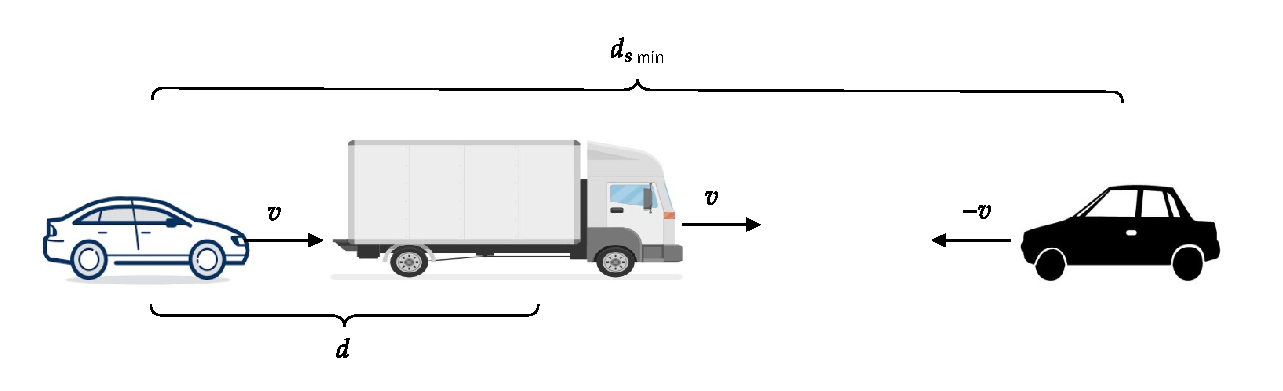
\includegraphics[width=0.8\linewidth]{diagram1}}

		Para encontrar o tempo de ultrapassagem $ t_u $, podemos fazer $ s(t_u)=\int_{0}^{t_u}\sbr{\int_{0}^{t}a(\tau)\dif\tau}\dif t\overset{!}{=}2d $ onde $ s(t) $ é o deslocamento no tempo $ t $ e $ a(t) $ é a aceleração do veículo que deseja fazer a ultrapassagem (considerada constante e de módulo $ a(t)=a_{\text{máx}}=\SI{3}{\meter\per\second\squared} $).
		Resolvendo, temos
		\begin{align*}
			s(t_u) & =\int_{0}^{t_u}\sbr{\int_{0}^{t}a(\tau)\dif\tau}\dif t=\int_{0}^{t_u}\sbr{\int_{0}^{t}a_{\textup{máx}}\dif\tau}\dif t \\
			       & =\int_{0}^{t_u}\eval{\del{a_{\textup{máx}}\,\tau}}_{0}^{t}\dif t=\int_{0}^{t_u}a_{\textup{máx}}\,t\dif t              \\
			       & =\eval{\del{\dfrac{1}{2}a_{\textup{máx}}\,t^{2}}}_{0}^{t_u}=\dfrac{a_{\textup{máx}}}{2}t_u^{2}\overset{!}{=}2d
		\end{align*}
		Daí, temos $ t_u=2\sqrt{d/a_{\textup{máx}}} $.

		Considerando o tempo mínimo de uma ultrapassagem segura como $ t_s=t_u=2\sqrt{d/a_{\textup{máx}}} $, teremos a distância mínima para a ultrapassagem como a integral da velocidade relativa $ \vec{v_{rel}} $ entre os dois veículos no intervalo de tempo considerado.

		Estando os dois indo em sentidos opostos, com velocidade de módulo $ v $, temos:
		\[ \begin{cases}
				v_1(t)=v+\displaystyle\int_{0}^{t}a(\tau)\dif \tau \\
				v_2(t)=-v
			\end{cases} \]
		Logo,
		\begin{align*}
			v_{rel}(t) & =v_1(t)-\vec{v_2}(t)=v+\int_{0}^{t}a(\tau)\dif \tau-\del{-v} \\
			           & =2v+\int_{0}^{t}a(\tau)\dif \tau
		\end{align*}
		Portanto,
		\begin{align*}
			s(t_s) & =\int_{0}^{t_s}v_{rel}=\int_{0}^{t_s}2v+\sbr{\int_{0}^{t}a(\tau)\dif\tau}\dif t                                                                                              \\
			\intertext{substituindo os valores:}
			       & =\int_{0}^{t_s}2v+a_{\textup{máx}}\,t\dif t=\eval{\del{2\dfrac{80}{\num{3.6}}t+\dfrac{3}{2}t^{2}}}_{0}^{t_s=2\sqrt{d/a_{\textup{máx}}}=\num[parse-numbers=false]{2\sqrt{5}}} \\
			       & =\dfrac{160}{3.6}(2\sqrt{5})+\dfrac{3}{2}(2\sqrt{5})^{2}\approx\SI{228.76}{\meter}
		\end{align*}
	\end{solution}

	\question
	Um trem com aceleração máxima $ a $ e desaceleração máxima $ f $ (magnitude da aceleração de freamento) tem de percorrer uma distância $ d $ entre duas estações. O maquinista pode escolher entre (a) seguir com a aceleração máxima até certo ponto e a partir daí frear com desaceleração máxima, até chegar, ou; (b) acelerar até uma certa velocidade, mantê-la constante durante algum tempo e depois frear até a chegada. Mostre que a primeira opção é a que minimiza o tempo de percurso (sugestão: utilize gráficos $ v\times t  $) e calcule o tempo mínimo de percurso em função de $ a $, $ f $ e $ d $.

	\by{João Vitor \& myself}
	\begin{solution}
		Sendo $ d $ a área do gráfico, no caso mais geral (trapézio), temos
		\begin{equation}\label{eq:dgraf}
			d=\dfrac{1}{2}v_{max}\del{t_f+\del{t_b-t_a}}.
		\end{equation}

		Sabendo que o trem começa e termina a viagem com $ v=0 $, podemos usar a definição de aceleração média para encontrar duas relações
		\begin{gather}
			v_{max}=a\,t_a\quad\text{e}\\
			-v_{max}=-f\del{t_f-t_b}
		\end{gather}
		isolando os tempos e somando as duas equações, temos
		\begin{align}
			\dfrac{v_{max}}{a}+\dfrac{v_{max}}{f} & =t_f-t_b+t_a\nonumber                                     \\
			v_{max}\del{\dfrac{f+a}{f\,a}}        & =t_f-\Delta t,\quad \Delta t=t_b-t_a\nonumber             \\
			v_{max}                               & =\del{t_f-\Delta t}\dfrac{f\,a}{f+a}.\label{eq:vmaxtrain}
		\end{align}

		Substituindo em \ref{eq:dgraf} e isolando $ t_f $, temos
		\begin{align*}
			d                    & =\dfrac{1}{2}\del{t_f-\Delta t}\del{t_f+\Delta t}\dfrac{f\,a}{f+a} \\
			t_f^{2}-\Delta t^{2} & =\dfrac{2d\del{f+a}}{f\,a}                                         \\
			t_f                  & =\sqrt{\dfrac{2d\del{f+a}}{f\,a}+\Delta t^{2}}.
		\end{align*}
		Sendo o primeiro termo da raiz uma constante, denotemos ele por $ C $. Vamos, então, derivar $ t_f $ com respeito à $ \Delta t $ e igualar a zero, a fim de encontrar um mínimo:
		\[ \dod{t_f}{\Delta t}=2\Delta t\dfrac{1}{2}\dfrac{1}{\sqrt{C+\Delta t^{2}}}=0\implies \Delta t=0 \]
		Dessa forma, sabemos que $ t_f $ é mínimo quando $ t_a=t_b $, e o trecho para o qual $ v= $const. não existe.

		\newcommand{\ag}{0.7}

		\begin{multi}

			\centering
			\begin{tikzpicture}[x=0.6cm,y=0.6cm]
				\begin{axis}[
						title={\footnotesize Velocidade por tempo (caso geral)},
						axis lines=middle,
						every axis y label/.style={at={(current axis.north west)},above=0mm,xshift=5.5mm},
						every axis x label/.style={at={(current axis.right of origin)},anchor=west},
						ylabel={$ v $},
						xlabel={$ t $},
						ytick={0},
						xtick={0},
						xmin=-1,xmax=12,
						ymin=-0.5,ymax=10,
					]
					\path[name path=axis] (axis cs:0,0) -- (axis cs:10,0);

					\addplot[name path=f,black,domain=0:4] {2*x};
					\addplot[name path=g,black,domain=4:6] {8};
					\addplot[name path=h,black,domain=6:10] {-2*x+20};

					\addplot [thick,color=blue,fill=blue,fill opacity=0.05]
					fill between[of=f and axis,soft clip={domain=0:4},];
					\addplot [thick,color=blue,fill=blue,fill opacity=0.05]
					fill between[of=g and axis,soft clip={domain=4:6},];
					\addplot [thick,color=blue,fill=blue,fill opacity=0.05]
					fill between[of=h and axis,soft clip={domain=6:10},];

					\coordinate (ti) at (axis cs:0,0);
					\coordinate (ta) at (axis cs:4,0);
					\coordinate (tb) at (axis cs:6,0);
					\coordinate (tf) at (axis cs:10,0);

					\coordinate (va) at (axis cs:4,8);
					\coordinate (vb) at (axis cs:6,8);

					\coordinate (vc) at (axis cs:0,8);

					\coordinate (A) at (axis cs:5,4);
				\end{axis}
				\filldraw (ta) circle (1pt) node[below left] {$ t_a $};
				\filldraw (tb) circle (1pt) node[below right] {$ t_b $};
				\filldraw (tf) circle (1pt) node[below right] {$ t_f $};

				\draw[dashed] (ta) -- (va) (tb) -- (vb);
				\draw[densely dashed] (ti) -- +(0,-\ag) (ta) -- +(0,-\ag) (tb) -- +(0,-\ag) (tf) -- +(0,-\ag);
				%		\draw[dashed] (O-|max) -- (max);
				\draw[decorate,decoration={brace,mirror,amplitude=10pt,raise=0pt}] (ti) ++(0,-\ag) -- node[below=10pt] {$ v_a(t) $} ($ (ta)+(0,-\ag) $);
				\draw[decorate,decoration={brace,mirror,amplitude=10pt,raise=0pt}] (ta) ++(0,-\ag) -- node[below=10pt] {$ v_c(t) $} ($ (tb)+(0,-\ag) $);
				\draw[decorate,decoration={brace,mirror,amplitude=10pt,raise=0pt}] (tb) ++(0,-\ag) -- node[below=10pt] {$ v_f(t) $} ($ (tf)+(0,-\ag) $);

				\node at (A) {$ d $};
			\end{tikzpicture}

			\nextcol

			\centering

			\begin{tikzpicture}[x=0.6cm,y=0.6cm]
				\begin{axis}[
						title={\footnotesize Velocidade por tempo (caso para $ \min t_f $)},
						axis lines=middle,
						every axis y label/.style={at={(current axis.north west)},above=0mm,xshift=5.5mm},
						every axis x label/.style={at={(current axis.right of origin)},anchor=west},
						ylabel={$ v $},
						xlabel={$ t $},
						ytick={0},
						xtick={0},
						xmin=-1,xmax=12,
						ymin=-0.5,ymax=12,
					]
					\path[name path=axis] (axis cs:0,0) -- (axis cs:10,0);

					\addplot[name path=f,black,domain=0:5] {2*x};
					\addplot[name path=h,black,domain=5:10] {-2*x+20};

					\addplot [thick,color=blue,fill=blue,fill opacity=0.05]
					fill between[of=f and axis,soft clip={domain=0:5},];
					%		\addplot [thick,color=blue,fill=blue,fill opacity=0.05]
					%		fill between[of=g and axis,soft clip={domain=4:6},];
					\addplot [thick,color=blue,fill=blue,fill opacity=0.05]
					fill between[of=h and axis,soft clip={domain=5:10},];

					\coordinate (ti) at (axis cs:0,0);
					\coordinate (ta) at (axis cs:5,0);
					\coordinate (tf) at (axis cs:10,0);

					\coordinate (va) at (axis cs:5,10);
					\coordinate (A) at (axis cs:4,4);
				\end{axis}
				\filldraw (ta) circle (1pt) node[below left] {$ t_a $};
				\filldraw (tf) circle (1pt) node[below right] {$ t_f $};

				\draw[dashed] (ta) -- (va);
				\draw[densely dashed] (ti) -- +(0,-\ag) (ta) -- +(0,-\ag) (tf) -- +(0,-\ag);
				\draw[decorate,decoration={brace,mirror,amplitude=10pt,raise=0pt}] (ti) ++(0,-\ag) -- node[below=10pt] {$ v_a(t) $} ($ (ta)+(0,-\ag) $);
				\draw[decorate,decoration={brace,mirror,amplitude=10pt,raise=0pt}] (ta) ++(0,-\ag) -- node[below=10pt] {$ v_f(t) $} ($ (tf)+(0,-\ag) $);

				\node at (A) {$ d $};
			\end{tikzpicture}
		\end{multi}

		Assumindo o caso onde $ t_f $ é mínimo,
		\begin{equation}\label{eq:q8tf}
			d=\dfrac{v_{max}\,t_f}{2}\implies t_f=\dfrac{2d}{v_{max}}
		\end{equation}

		%		\begin{multi}[2][t]
		Para um movimento acelerado, dada uma velocidade inicial $ v_0 $, uma velocidade final $ v $ e uma aceleração qualquer $ a $, temos $ t=(v-v_0)/a $. Para um dado deslocamento $ d $, temos
		\begin{align}
			d     & =v_0\,t+\dfrac{1}{2}a\,t^{2}\nonumber                                               \\ &=v_0\dfrac{\del{v-v_0}}{a}+\dfrac{1}{2}a\del{\dfrac{\del{v-v_0}}{a}}^{2}\nonumber\\
			      & =\dfrac{2v_0\del{v-v_0}+\del{v-v_0}^{2}}{2a}\nonumber                               \\
			      & =\dfrac{2v_0\,v-2v_0^{2}+v^{2}-2v\,v_0+v_0^{2}}{2a}\nonumber                        \\
			2a\,d & =v^{2}-v_0^{2}\quad\text{\textit{The infamous Torricelli equation.}}\label{eq:torr}
		\end{align}

		Sendo $ d=d_a+d_f $ também, onde $ d_a $ e $ d_f $ são as distâncias percorridas durante a aceleração $ a $ e a aceleração $ f $, respectivamente. Substituindo em \ref{eq:torr}, temos
		\begin{gather*}
			v_{max}^{2}-0^{2}=2a\,d_a\implies d_a=\dfrac{v_{max}^{2}}{2a}\\
			0^{2}-v_{max}^{2}=-2f\,d_f \implies d_f=\dfrac{v_{max}^{2}}{2f}
		\end{gather*}
		Portanto
		\begin{align*}
			d           & =d_a+d_f=\dfrac{v_{max}^{2}}{2a}+\dfrac{v_{max}^{2}}{2f}                      \\
			d           & =\dfrac{v_{max}^{2}\del{f+a}}{2a\,f}                                          \\[1em]
			v_{max}^{2} & =\dfrac{2a\,f\,d}{f+a}                                                        \\
			v_{max}     & =\sqrt{\dfrac{2a\,f\,d}{f+a}}\quad\text{Pois a velocidade deve ser positiva.}
		\end{align*}
		Substituindo em \ref{eq:q8tf}, temos:
		\begin{align*}
			t_f & =\dfrac{2d}{\sqrt{\dfrac{2a\,f\,d}{f+a}}}=2d\sqrt{\dfrac{f+a}{2a\,f\,d}}      \\
			    & t_f=\sqrt{\dfrac{4d^{2}\del{f+a}}{2a\,f\,d}}=\sqrt{\dfrac{2d\del{f+a}}{a\,f}}
		\end{align*}
		\paragraph{Nota:} Repare que, sendo $ \Delta t=0 $ no caso do tempo mínimo, bastaria substituir \ref{eq:vmaxtrain} em \ref{eq:q8tf} para encontrar o mesmo resultado.

	\end{solution}

	\clearpage

	\question
	Um foguete para pesquisas meteorológicas é lançado verticalmente para cima. O combustível, que lhe imprime uma aceleração de $ \num{1.5}g $ ($ g $ é a aceleração da gravidade) durante o período de queima, esgota-se após
	$ 1/2 $ minuto.

	\begin{parts}
		\part
		Qual seria a altitude máxima atingida pelo foguete, se pudéssemos desprezar a resistência do ar?

		\begin{solution}

			%			\correctspacing
			\begin{multi}
				Para encontrar a altura máxima devemos encontrar $ h(t_s) $, onde $ t_s $ é o tempo de subida do foguete, devemos resolver $ v(t)\overset{!}{=}0 $, pois neste momento teremos a inversão do sentido da velocidade do foguete, que deve ter alcançado sua altitude máxima. Sendo a velocidade do foguete $ v(t) $ composta por duas acelerações (da gravidade $g$ e da queima do combustível $a_c$), as quais podemos descrever por:
				\[ \begin{cases}
						a_c(t)=\num{1.5}g \\
						g(t)=-g
					\end{cases} \]
				Integrando ambas com respeito ao tempo $ t $ e somando-as, encontramos a velocidade $ v(t_s) $:

				\nextcol

				\begin{align}
					v(t) & =\int_{0}^{t}\del{a_c(t')+g(t')}\dif t'\nonumber                            \\
					     & =\int_{0}^{30}\num{1.5}g \dif t' + \int_{30}^{t_s}-g \dif t'\nonumber       \\
					     & =\eval{\del{\num{1.5}g\,t'}}_{0}^{30}+\eval{\del{-g\,t'}}_{30}^{t}\nonumber \\
					     & =g\del{45-\del{t-30}}\nonumber                                              \\
					v(t) & =g\del{75-t}\label{eq:ex9.1}
				\end{align}
				Para encontrar o tempo de subida $ t_s $, basta fazermos $ v(t_s)=0 $:
				\[ g\del{75-t_{s}}=0\implies t_s=\SI{75}{\second} \]
			\end{multi}

			A partir disso podemos encontrar o deslocamento $ s(t=t_s) $ integrando a velocidade $ v(t) $ com respeito a $ t $:
			\begin{align*}
				s(t_s) & =\int_{0}^{t_s}v(t)\dif t                                                                                                \\
				       & =\int_{0}^{30}\sbr{\int_{0}^{t}a_c(\tau)\dif\tau}\dif t+\int_{30}^{t_s=\SI{75}{\second}}g\del{75-t}\dif t                \\
				\intertext{fazendo $ u=t-30\implies \dif u=\dif t $, temos}
				       & =g\del{\int_{0}^{30}\num{1.5}t\dif t
				+\int_{0}^{45}75-(u+30)\dif u}                                                                                                    \\
				       & =g\del{\eval{\del{\dfrac{\num{1.5}}{2}t^{2}}}_{0}^{30}+\eval{\del{45u-\dfrac{1}{2}u^{2}}}_{0}^{45}}                      \\
				       & =g\del{\dfrac{\num{1.5}}{2}30^{2}+45\cdot45-\dfrac{45^{2}}{2}}=g\dfrac{45\cdot\del{30+2\cdot45-45}}{2}                   \\
				s(t_s) & =\dfrac{45\cdot75}{2}g \approx \SI{16.5}{\kilo\meter} \quad (\text{Considerando }g=\SI{9.81}{\meter\per\second\squared})
			\end{align*}
		\end{solution}

		\clearpage

		\part
		Com que velocidade (em \si{\meter\per\second} e \si{\kilo\meter\per\hour}) e depois de quanto tempo, ele voltaria a atingir o solo?
		\begin{solution}
			Para encontrar o momento em que o foguete atinge o solo novamente, devemos encontrar $ s(t)=0, t>0 $. Podemos adotar um novo $ s(t+75)=s_q(t) $, onde consideramos apenas a queda do foguete. Podemos descrever $ s_q(t) $ como
			\begin{align*}
				s_q(t) & =s(75)+\int_{0}^{t}v_q(\tau)\dif\tau                 \\
				       & =s(75)+\int_{0}^{t}\int_{0}^{\tau}-g \dif t'\dif\tau \\
				       & =s(75)+\int_{0}^{t}-g\,\tau\dif \tau                 \\
				       & =s(75)-\dfrac{g}{2}\del{t^{2}}\overset{!}{=}0
			\end{align*}
			Resolvendo, temos:
			\begin{align*}
				\dfrac{45\cdot75}{2}g & =\dfrac{1}{2}g(t^{2})\implies                \\
				t                     & =\sqrt{45\cdot75} \approx\SI{58.09}{\second}
			\end{align*}


			Utilizando a equação \ref{eq:ex9.1}, para $ t_t=\num{58.09}+75=\SI{133.09}{\second} $ e $ g=\SI{9.81}{\meter\per\second\squared} $, temos:
			\[ |v(\num{133.09})|=|g\del{75-\num{133.09}}|=|\num{-58.09}g|\approx\SI{569.86}{\meter\per\second}\approx\SI{2051.51}{\kilo\meter\per\hour} \]

			%		\begin{multi}
			%			\paragraph{Nota:} a solução $ s(0)=0=s(90) $ é consonante com a resolução do item (a) $ s_{\text{máx}}=s(45) $ por conta da simetria do gráfico de uma função quadrática.
			%			
			%			\nextcol
			%			
			%			\centering
			%			\begin{tikzpicture}
			%			\begin{axis}[
			%			title={Posição por tempo},
			%			axis lines=middle,
			%			every axis x label/.style={at={(current axis.right of origin)},anchor=west},
			%			every axis y label/.style={at={(current axis.north west)},above right=2mm},
			%			ylabel={$ s $},
			%			xlabel={$ t $},
			%			ytick={0,200,...,1000},
			%			xtick={0,10,...,90},
			%			xmin=-5,xmax=95,
			%			ymin=-100,ymax=1100,
			%			]
			%			\addplot[black,domain=-2:92] {-0.5*x^2 + 45*x};
			%			\coordinate (O) at (axis cs:0,0);
			%			\coordinate (max) at (axis cs:45,1012.5);
			%			\coordinate (S) at (axis cs:90,0);
			%			\end{axis}
			%			\draw[dashed] (O-|max) -- (max);
			%			\draw[decorate,decoration={brace,mirror,amplitude=10pt,raise=0pt}] (O) ++(0,-0.8) -- node[below=10pt] {$ d $} ($ (O-|max)+(0,-0.8) $);
			%			\draw[decorate,decoration={brace,mirror,amplitude=10pt,raise=0pt}] ($ (O-|max)+(0,-0.8) $) -- node[below=10pt] {$ d $} ($ (S)+(0,-0.8) $);
			%			\end{tikzpicture}
			%		\end{multi}
		\end{solution}
	\end{parts}

	\clearpage

	\question
	Um Boeing 777 está se dirigindo à porta de desembarque em um aeroporto após aterrissagem. Em um determinado instante o avião se encontra na posição da figura \ref{fig:plane}, onde as rodas dianteiras estão alinhadas com a linha amarela que ele deve seguir até o ponto de estacionamento, enquanto as rodas traseiras estão posicionadas de forma a rodar o corpo do avião para alinhá-lo também com a mesma linha. Mostre que o alinhamento nunca poderá ser perfeito. Admita que a distância entre as rodas dianteiras e traseiras seja de \SI{30}{\meter}, que o avião esteja se deslocando a \SI{5}{\meter\per\second} e que inicialmente a distância das rodas traseiras da linha amarela seja de \SI{10}{\meter}. Quanto tempo leva o avião até que a distância das rodas traseiras da linha amarela seja de \SI{10}{\centi\meter}? Qual o deslocamento do avião durante esse tempo?

	\begin{figure}[h]
		\centering
		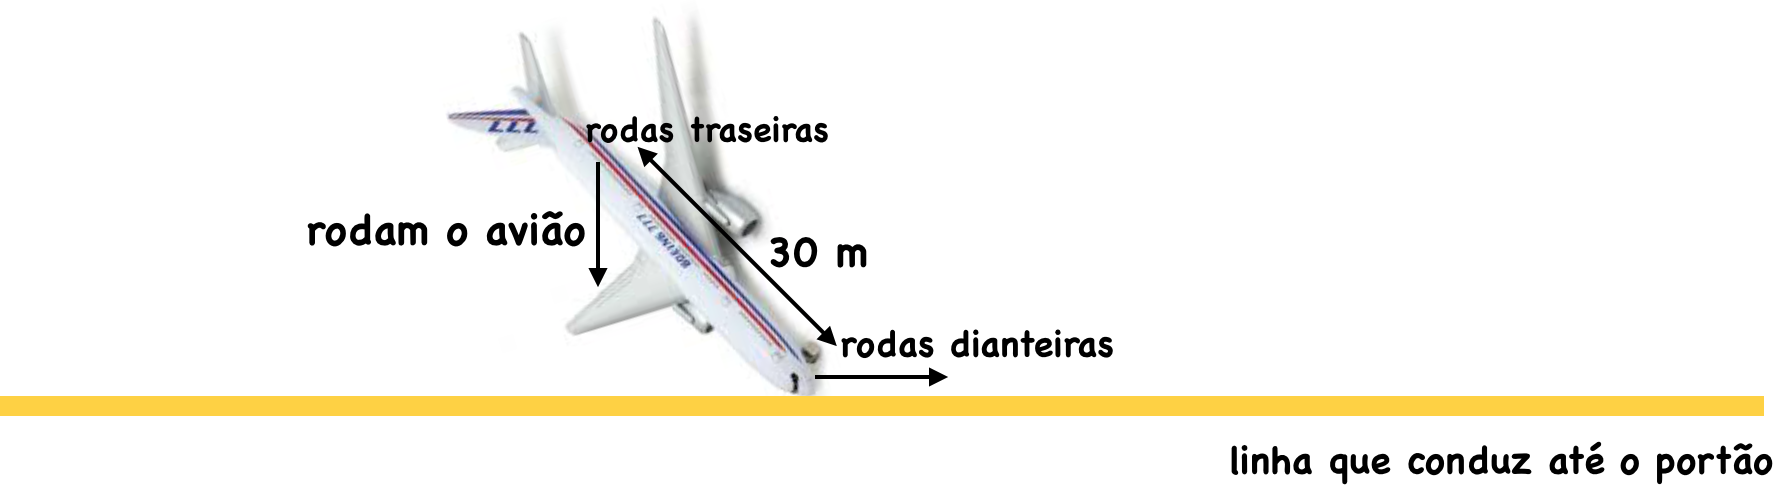
\includegraphics[width=1\linewidth]{screenshot001}
		\caption{Avião se posicionando para entrar no portão de desembarque.}
		\label{fig:plane}
	\end{figure}

	\by{Anahí \& monitores}
	\begin{solution}

		\correctspacing
		\begin{multi}
			Montando o diagrama ao lado, e assumindo que a velocidade das rodas traseiras $ v_t(t) $ seja constante e de módulo \SI{5}{\meter\per\second}, e que $ v_d(t) $ seja a velocidade das rodas dianteiras, temos.
			\begin{gather}
				\cos\theta=\dfrac{x(t)}{L}\label{eq:q10cos}\\
				\sin\theta=\dfrac{y(t)}{L}\label{eq:q10sin}
			\end{gather}

			\nextcol
			\centering
			\begin{tikzpicture}[x=2cm,y=2cm]
				\draw[->] (-0.25,0) -- (2.5,0) node[right] {$ x $};
				\draw[->] (0,-0.25) -- (0,2) node[above] {$ y $};

				\coordinate (O) at (0,0);
				\coordinate (t) at (0,1.5);
				\coordinate (d) at (1.5,0);

				\draw[decorate,decoration={brace,amplitude=5pt,raise=5pt}] (O) -- node[left=10pt] {$ y(t) $} (t);
				\draw[decorate,decoration={brace,amplitude=5pt,raise=5pt}] (d) -- node[below=10pt] {$ x(t) $} (O);

				\draw (t) -- node[rotate=-45,above] {$ L=\SI{30}{\meter} $} (d);
				\draw[-Latex,red] (t) -- node[rotate=-45,above] {$ v_t $} +(0.5,-0.5);
				\draw[-Latex,red] (d) -- node[above] {$ v_d $} +(0.5,0);


				\pic[draw=black,fill=gray!50, angle radius=15pt,angle eccentricity=1,"$ \theta $" {xshift=-4pt,yshift=2pt}] {angle=t--d--O};
				\filldraw (t) circle (1pt) (d) circle (1pt);

			\end{tikzpicture}

		\end{multi}

		e daí, encontrando a velocidade com que a posição vertical das rodas traseiras varia, temos:
		\begin{align*}
			\dot{y} & =-v_t\,\sin\theta    \\
			        & =-\dfrac{v_t}{L}y(t)
		\end{align*}
		que é uma equação diferencial, cuja resolução recai em:
		\[ y(t)=A\,\exp{\del{-\dfrac{v_t}{L}t}} \]

		Analisando a condição inicial, dada no problema, temos
		\[ y(0)=10\implies A=10 \]
		o que nos dá a posição com forma geral:
		\begin{equation}\label{eq:q10yt}
			y(t)=10\,\exp{\del{-\dfrac{t}{6}}}
		\end{equation}

		Sabendo que a função exponencial pura possui assíntota no eixo $ x $ e, portanto, as rodas traseiras nunca estarão perfeitamente alinhadas às dianteiras.

		Para encontrar o tempo até que as rodas traseiras tenham \SI{10}{\centi\meter} de distância da linha amarela, podemos igualar \ref{eq:q10yt} ao valor desejado, resolvendo para o tempo
		\begin{align*}
			y(t)                           & =10^{-1}                            \\
			10\,\mathrm{e}^{-\dfrac{t}{6}} & =10^{-1}                            \\
			-\dfrac{t}{6}                  & =\ln 10^{-2}                        \\
			t                              & =12\ln10\approx\SI{27.631}{\second}
		\end{align*}

		Para encontrar a distância percorrida na horizontal nesse tempo, devemos encontrar a função $ x_d(t) $.

		Sabemos que $ L $ é constante, e que sempre vale
		\[ L^{2}=x^{2}(t)+y^{2}(t)\implies x(t)=\sqrt{L^{2}-y^{2}(t)} \]
		Também temos que:
		\[ x(t)=x_d(t)-x_t(t) \]
		igualando as duas e derivando
		\begin{align*}
			\sqrt{L^{2}-y^{2}(t)}                                                             & =x_d(t)-x_t(t)\implies                               \\
			\del{\sqrt{L^{2}-y^{2}(t)}}'                                                      & =\del{x_d(t)-x_t(t)}'                                \\
			u'\del{u^{1/2}}'                                                                  & =x_d'(t)-x_t'(t)\quad\text{onde }u=L^{2}-y^{2}(t)    \\
			\del{\dod{}{t}\sbr{L^{2}-y^{2}(t)}}\dfrac{1}{2}\del{L^{2}-y^{2}(t)}^{-1/2}        & =v_d(t)-v_t(t)\,\cos\theta                           \\
			\del{\dod{v}{t}\dod{}{v}\sbr{L^{2}-v^{2}}}\dfrac{1}{2}\del{L^{2}-y^{2}(t)}^{-1/2} & =v_d(t)-v_t(t)\dfrac{x(t)}{L}\quad\text{onde }v=y(t) \\
			\dod{y}{t}\del{-2y(t)}\dfrac{1}{2}\del{L^{2}-y^{2}(t)}^{-1/2}                     & =v_d(t)-\dfrac{1}{6}x(t)
		\end{align*}
		\begin{equation}\label{eq:q10ydot}
			-y(t)\dot{y}\del{L^{2}-y^{2}(t)}^{-1/2}=v_d(t)-\dfrac{\sqrt{L^{2}-y^{2}(t)}}{6}
		\end{equation}
		Derivando \ref{eq:q10yt}, temos
		\[ \dot{y}(t)=-\dfrac{10}{6}\,\exp{\del{-\dfrac{t}{6}}}=-\dfrac{1}{6}y(t) \]
		Substituindo em \ref{eq:q10ydot} e isolando $ v_d(t) $
		\begin{align*}
			v_d(t) & =\dfrac{\sqrt{L^{2}-y^{2}(t)}}{6}-y(t)\del{-\dfrac{1}{6}y(t)}\del{L^{2}-y^{2}(t)}^{-1/2} \\
			       & =\dfrac{\del{\sqrt{L^{2}-y^{2}(t)}}^{2}+y^{2}(t)}{6\sqrt{L^{2}-y^{2}(t)}}                \\
			       & =\dfrac{L^{2}}{6\sqrt{L^{2}-y^{2}(t)}}
		\end{align*}
		Integrando com respeito a $ t $, temos
		\begin{align*}
			\int v_d(t)\dif t & =x_d(t)=\int\dfrac{L^{2}}{6\sqrt{L^{2}-y^{2}(t)}}\dif t                        \\
			\intertext{fazendo $ y=y(t)\implies\dif y=-y(t)/6 \dif t $}
			                  & =\int\dfrac{L^{2}}{6\sqrt{L^{2}-y^{2}}} \del{-\dfrac{6}{y}}\dif y              \\
			                  & =-\int\dfrac{L^{2}}{y\sqrt{L^{2}-y^{2}}}\dif y                                 \\
			\intertext{fazendo $ y=L\,\sin\varphi\implies \dif y=L\,\cos\varphi\dif\varphi $}
			                  & =-\int\dfrac{L^{2}\del{\cancel{L}\,\cos\varphi}}
			{\del{\cancel{L}\,\sin\varphi}\sqrt{L^{2}-\del{L\,\sin\varphi}^{2}}}\dif\varphi                    \\
			                  & =-\int\dfrac{L^{2}\cos\varphi}
			{\sin\varphi\sqrt{L^{2}\del{1-\sin^{2}\varphi}}}\dif\varphi                                        \\
			                  & =-\int\dfrac{L^{2}\cos\varphi}
			{\sin\varphi\sqrt{\del{L\cos\varphi}^{2}}}\dif\varphi                                              \\
			                  & =-\int\dfrac{L^{2}\cancel{\cos\varphi}}
			{L\sin\varphi\,\cancel{\cos\varphi}}\dif\varphi                                                    \\
			                  & =-L\int\dfrac{1}
			{\sin\varphi}\dif\varphi                                                                           \\
			                  & =-L\,\ln{\envert{\csc\varphi-\cot\varphi}}+C                                   \\
			                  & =-L\,\ln{\envert{\dfrac{1}{\sin\varphi}-\dfrac{\cos\varphi}{\sin\varphi}}}+C   \\
			                  & =-L\,\ln{\envert{\dfrac{L}{y(t)}\del{1-\sqrt{1-\del{\dfrac{y(t)}{L}}^{2}}}}}+C
		\end{align*}
		Tomando a integral definida e substituindo os valores, temos
		\begin{align*}
			\int_{0}^{t=27.631} v_d(\tau)\dif \tau & =x(t=27.631)=\left. \del{-30\,\ln{\envert{\dfrac{30}{y(\tau)}\del{1-\sqrt{1-\del{\dfrac{y(\tau)}{30}}^{2}}}}}+C}\right|_{0}^{t=27.631} \\
			                                       & =-30\,\ln{\envert{\dfrac{30}{10^{-1}}\del{1-\sqrt{1-\del{\dfrac{10^{-1}}{30}}^{2}}}}}\approx \SI{191.91}{\meter}
		\end{align*}
		que é o deslocamento horizontal do avião.

	\end{solution}

\end{questions}
\end{document}
